\chapter{Discrete modeling of the dynamics on the spatially non-uniform membrane}

\label{non_uniform_membrane}

The work presented in this chapter has been published in the paper of Kiselev et al. \cite{Kiselev2011} and has been done by me, except the sections where the work of other authors is explicitly mentioned.

In the previous chapter the peptide lateral dynamics on the uniform membrane was considered. However, the cell membrane is a medium with the ever changing composition. Recent experimental data indicate that various lipid-modifying enzymes can be rapidly recruited and activated on the membrane \cite{Brown1998,Chatah2001}. Lipid kinases, phosphatases, and some phospholipases alter the lipid charge by adding or removing phosphate groups or using other specific mechanisms. For instance, the monovalent phosphatidic acid (PA) can be produced from the neutral PC lipid by the action of the phospholipase D \cite{Cazzolli2006,Rizzo2002}. PIP$_2$ can be rapidly produced by phosphatidylinositol 4-phosphate 5-kinase (PIP5K) by phosphorylation of PI(4)P lipid in a large number of cell signaling events \cite{Bout2009,Kwiatkowska2010a}. Constant production of the negatively charged lipids on the membrane can generate a gradient of these lipids in the vicinity of the lipid producing enzyme. As a consequence, the associated gradients of the surface charge can generate a temporary electrostatic potential along the membrane. Since the PDs are located in the closest vicinity of the membrane \cite{Ben-Tal1996}, presumably, they can perceive and respond to the changes in the electrostatic potential. To test this hypothesis, I modified the original MCA by introducing a gradient of the negatively charged monovalent lipids along the membrane width. Particularly, to create a stable gradient, charged lipids are inserted periodically on the left boundary and removed from the lattice once they approach the right boundary. After a large number of iterations (at least 20000) when the gradient becomes stable, the peptide is inserted into the middle of the lattice and its lateral displacement is monitored. Note, that the concentration of the monovalent lipids in the middle of the membrane lattice depends on the value of the lipid gradient, consequently changing the electrostatic properties of the PD (the averaged occupation by monovalent lipids, the peptide total charge etc.). To achieve the constant concentration of monovalent lipids at the lattice center with varying values of the gradient, I introduced two lipid species with the same charge (-1) but distinct boundary conditions. The gradient was generated in the spatial distribution of one species, whereas the other exhibited homogeneous distribution owing to the periodic boundary conditions.

At the time of the peptide insertion into the membrane lattice in the MCA the lipid dynamics is already at the steady state, i.e. the sum of all lipid fluxes at any point of the lattice on average equals 0. Thus, I neglect possible hydrodynamic effects in the peptide diffusion, caused by the lipid fluxes on the membrane.

\section{Analytical estimation of the PD drift}

\label{peptide_velocity_estimation}

To analyze the hypothesis of the PD response to the gradient of the electrostatic potential I use a mean-field continuous estimation of the peptide velocity, derived by Davide Marenduzzo. He considers a continuous distribution of lipids, described by a density field $\rho(\vec{\mathbf{r}})$, in the piece of the membrane with the characteristic size $L_d\gg l_p$ ($l_p$ is the characteristic peptide size). The peptide is located at $\vec{\mathbf{r}}^*$ and interacts with negatively charged membrane lipids according to eq. \eqref{yukawa_potential}. The total interaction potential between the peptide and all membrane lipids can be described as follows:
\begin{equation}
\label{Davide_potental}
 V(\vec{\mathbf{r}}^*) \simeq \int d\vec{\mathbf{r}}\frac{Zq}{4\pi\varepsilon\varepsilon_0} \rho(\vec{\mathbf{r}}^*+\vec{\mathbf{r}})\frac{e^{-r/\lambda}}{r}
\end{equation}
where the sum over all discrete lipid positions is approximated by the integral over the surface, $q$ is a charge of a single lipid, $Z$ is the peptide charge. The peptide will experience the force created by the gradient of the potential \eqref{Davide_potental}:
\begin{equation}
\label{Davide_force1}
 \vec{\mathbf{f}}(\vec{\mathbf{r}}^*) = -\frac{\partial V(\vec{\mathbf{r}}^*)}{\partial \vec{\mathbf{r}}^*}
\end{equation}

If $\rho(\vec{\mathbf{r}})$ has a gradient on the membrane, substitution of eq. \eqref{Davide_potental} to eq. \eqref{Davide_force1} yields:
\begin{equation}
\label{Davide_force2}
 \vec{\mathbf{f}}(\vec{\mathbf{r}}^*) = -\frac{Zq}{4\pi\varepsilon\varepsilon_0} \int d\vec{\mathbf{r}} \hspace{0.05in} \vec{\mathbf{\nabla}}\rho(\vec{\mathbf{r}}^*+\vec{\mathbf{r}})\frac{e^{-r/\lambda}}{r}
\end{equation}

If the gradient of the lipid density is constant, i.e. if $\vec{\mathbf{\nabla}}\rho(\vec{\mathbf{r}}^*+\vec{\mathbf{r}}) \equiv \vec{\mathbf{\nabla}}\rho(\vec{\mathbf{r}}^*)$, then it can be taken out of the integral in eq. \eqref{Davide_force2}, providing the following:
\begin{equation}
 \label{Davide_force3}
 \vec{\mathbf{f}}(\vec{\mathbf{r}}^*) = -\frac{Zq}{4\pi\varepsilon\varepsilon_0} \hspace{0.05in} \vec{\mathbf{\nabla}}\rho(\vec{\mathbf{r}}^*) \int d\vec{\mathbf{r}}\hspace{0.05in} \frac{e^{-r/\lambda}}{r}
\end{equation}

Transforming to the polar coordinates, one can obtain:
\begin{equation}
  \label{Davide_force4}
 \vec{\mathbf{f}}(\vec{\mathbf{r}}^*) = -\frac{Zq}{4\pi\varepsilon\varepsilon_0} \hspace{0.05in} \vec{\mathbf{\nabla}}\rho(\vec{\mathbf{r}}^*) \int_0^{2\pi} d\theta \int_0^\infty r dr\hspace{0.05in} \frac{e^{-r/\lambda}}{r}
\end{equation}

Since the last integral in \eqref{Davide_force4} equals to $\lambda$, the final equation for the force, acting on the peptide, will have the following form:
\begin{equation}
  \label{Davide_force5}
 \vec{\mathbf{f}}(\vec{\mathbf{r}}^*) = -\frac{Zq}{2\varepsilon\varepsilon_0} \hspace{0.05in}\lambda \hspace{0.05in}\vec{\mathbf{\nabla}}\rho(\vec{\mathbf{r}}^*)
\end{equation}

Using Stokes-Einstein's relation, one can express the velocity of the peptide propelled by the force $\vec{\mathbf{f}}$ in a viscous (membrane) medium:
\begin{equation}
\label{Davide_velocity1}
 \vec{\mathbf{v}} = \frac{D_p}{k_BT}\vec{\mathbf{f}} = -\frac{Zq}{2\varepsilon\varepsilon_0} \frac{\lambda D_p \vec{\mathbf{\nabla}}\rho(\vec{\mathbf{r}}^*)}{k_BT}
\end{equation}
where $D_p$ is the peptide diffusion coefficient and $k_B$ is the Boltzmann's constant.

This velocity can be also expressed through the Bjerrum length:
\begin{equation}
\label{bjerrum_length0}
 l_B = \frac{e^2}{4\pi\varepsilon\varepsilon_0 k_BT}
\end{equation}
which represents the distance at which two ions with elementary charges interact with the energy $k_BT$. Thus, the velocity will have the following form:
\begin{equation}
\label{Davide_velocity2}
 \vec{\mathbf{v}} =  -2\pi\frac{Zq}{e^2} l_B \lambda D_p \vec{\mathbf{\nabla}}\rho(\vec{\mathbf{r}}^*)
\end{equation}

Eq. \eqref{Davide_velocity2} shows that in the mean-field approximation, when fluctuations of lipid density can be neglected, the charged peptide experiences a directional drift along the gradient of the lipid concentration with a constant velocity. The velocity of the drift is directly proportional to the peptide charge $Z$, its diffusion coefficient $D_p$, Debye length $\lambda$, the lipid charge $q$ and the value of the lipid gradient $\vec{\mathbf{\nabla}}\rho(\vec{\mathbf{r}}^*)$ at position $\vec{\mathbf{r}}^*$.

\section{Influence of the membrane hydrophobic core on the peptide drift}

The calculations, shown in this section, are done by Davide Marenduzzo.

In section \ref{peptide_velocity_estimation} the velocity of the peptide on the gradient of anionic lipids was derived without considering of the membrane hydrophobic core. However, due to hydrophobic properties of lipid tails the dielectric constant in the membrane core can be negligible compared to the one in the cytoplasm. This discontinuity of the dielectric constant at the membrane-water interface changes the nature of interaction between charged particles located close to this interface. To investigate how such a refinement impact on the results for the drift velocity of the peptide in a lipid gradient (eq. \eqref{Davide_velocity2}) one can follow the approach developed by Tzlil \cite{Tzlil2008} on the basis of the original work by Netz \cite{Netz1999}. Within this framework the electrostatic potential \eqref{yukawa_potential} is modified to account for the presence of the membrane hydrophobic core (the potential is calculated for the metallic half-space with negligible dielectric constant under the assumption of a finite dielectric constant in the rest of the space):
\begin{equation}
 V^h=\frac{qq'}{4\pi\varepsilon\varepsilon_0}\frac{e^{-\frac{\sqrt{r^2+4zz'}}{\lambda}}}{\sqrt{r^2+4zz'}}
\end{equation}
where $q$ and $q'$ are the charges of the interacting particles, $\lambda$ is the Debye length, $z$ and $z'$ are the distances of the
two charges $q$ and $q'$ from the membrane-water interface.

To estimate the distances $z$ and $z'$, one can use a recently calculated distances between the membrane-water interface and the charged headgroups of phospholipids \cite{Nymeyer2008}. In agreement with the previously published data, these distances are shown to be approximately 1 nm. Given the geometry of the MCA, $z$ and $z'$ are approximately equal and are both on the order of one Debye length ($\lambda\approx1$ nm).

Thus, the two dimensional integrals in eqs. \eqref{Davide_potental}, \eqref{Davide_force2}, \eqref{Davide_force3} and \eqref{Davide_force4}:
\begin{equation}
 \int_0^{2\pi} d\theta \int_0^\infty r dr \frac{e^{-r/\lambda}}{r}
\end{equation}
should be replaced with:
\begin{equation}
\label{new_integral}
 \int_0^{2\pi} d\theta \int_0^\infty r dr \Bigg[\frac{e^{-r/\lambda}}{r} + \frac{e^{-\frac{\sqrt{r^2+4z^2}}{\lambda}}}{\sqrt{r^2+4z^2}}\Bigg]
\end{equation}

Since the integration of the second term in the integral \eqref{new_integral} can still be analytically performed, the corrected expression of the peptide drift velocity \eqref{Davide_velocity2} will have the following form:
\begin{equation}
 \label{peptide_velocity_corrected}
 \vec{\mathbf{v}} =  -2\pi\frac{Zq}{e^2} l_B \lambda D_p \vec{\mathbf{\nabla}}\rho(\vec{\mathbf{r}}^*)(1+e^{-2z/\lambda})
\end{equation}

Eq. \eqref{peptide_velocity_corrected} contains the additional term $(1+e^{-2z/\lambda})$, compared to the original expression of the peptide velocity \eqref{Davide_velocity2}. The maximum value of this term is 2, corresponding to the situation when interacting charges are located directly on the membrane-water interface. However, under the assumption $z = z' = 1$ nm, described above, the correction $(1+e^{-2z/\lambda})$ is rather small (about 14\%) and therefore does not significantly change the results obtained by eq. \eqref{Davide_velocity2}.

\section{Peptide effective charge}

\label{description_peptide_effective_charge}

Due to the lipid demixing effect (see subsection \ref{lipid_demixing}) the nature of the peptide charge $Z$, introduced in the eq. \eqref{Davide_velocity2} for the peptide drift velocity, can be complicated. Indeed, the intrinsic charge of the peptide is always constant and equals +5. However, upon lipid demixing and consequent sequestration the introduced total peptide charge (see Fig. \ref{fig:total_peptide_charge}) can be significantly smaller and even become strongly negative (in the presence of PIP$_2$). Since in the MCA the peptide diffuses together with negatively charged lipids that are located directly underneath the peptide residues (according to the model assumption), the reduction of the total peptide charge should be reflected by $Z$. Moreover, due to the specific mechanism of the lipid moves (Kawasaki step, see subsection \ref{delta_energy_calculation}), the associated current of lipids, created by the peptide diffusion, in the direction opposite to the peptide drift should also be taken into account.

To include all translocating charges in $Z$, one should consider one peptide movement in details. I consider a binary PC/PS membrane and describe the peptide movement with respect to one peptide residue with the intrinsic charge +1. As the molar fraction of PS lipid, $\rho$, grows from 0\% to 100\%, the total charge of the residue decreases from +1 to 0, as shown by the dashed line in Fig. \ref{fig:effective_peptide_charge}, B. If the probability of the peptide residue being associated with PS is $p(\rho)$ then the total residue charge is $1-p(\rho)$. I denote the initial position of the residue before the movement as ``old'' and the final position of the residue after the movement as ``new''. Before the move the ``new'' position is occupied by PS lipid with the probability $\rho$ and the peptide residue in the ``old'' position is bound to a PS lipid with the probability $p(\rho)$. One can also assume that these two random events are independent of each other and thus mutual probabilities can be calculated as products of corresponding event probabilities. If the peptide residue is originally bound to a PS lipid, the movement of the residue is associated with the dragging of this lipid resulting in the Kawasaki ``swap'' with the lipid located in the ``new'' position. There are four possible scenarios of moving from the ``old'' to the ``new'' position (Fig. \ref{fig:effective_peptide_charge}, A):
\begin{figure}[!ht]
%\centering
%\scalebox{1.0}[1.0]
\begin{center}
  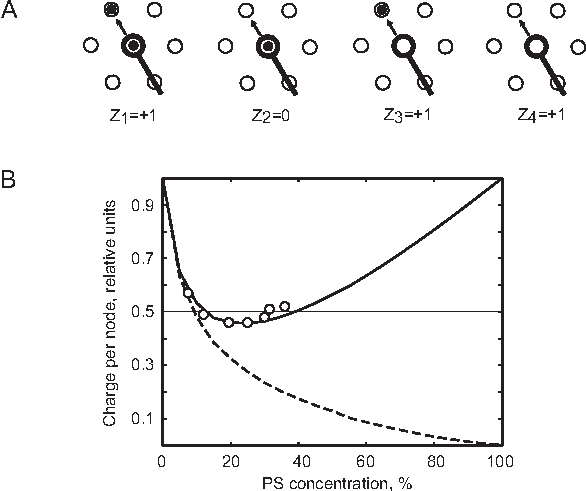
\includegraphics[scale=1.2]{../figures/effective_peptide_charge.pdf}
\end{center}
 \caption[Characteristic peptide charges]{Characteristic peptide charges (from \cite{Kiselev2011}). The value of the effective charge Z in eq. \eqref{Davide_velocity2} that translocates during the drift of the peptide is a weak function of the local PS concentration. (A) The four possible elementary translational moves of a peptide node (shown by thick line) projected onto the lipid lattice. Solid circle within the lipid lattice node represents a PS lipid. (B) The value predicted by eq. \eqref{effective_charge} (solid line) is compared to the simulation results (open circles). The total charge of the peptide together with the associated lipids is shown by the dashed line.}
\label{fig:effective_peptide_charge}
\end{figure}
\begin{enumerate}
 \item The peptide residue is bound to PS and the ``new'' position is also occupied by a charged PS lipid. In this case, the effective translocating charge is $Z_1=+1$ (the charge of the residue) and it occurs with the probability $P_1=p(\rho)\cdot\rho$;
 \item The peptide residue is bound to PS and the ``new'' position is occupied by a neutral PC lipid. In this case, the effective translocating charge is $Z_2=0$ (the charge of the residue plus the charge of the PS lipid) and it occurs with the probability $P_2=p(\rho)\cdot(1-\rho)$;
 \item The peptide residue is free of a PS lipid and the ``new'' position is occupied by a charged PS lipid. In this case, the effective translocating charge is $Z_3=+1$ (the charge of the residue) and it occurs with the probability $P_3=(1-p(\rho))\cdot\rho$;
 \item The peptide residue is free of a PS lipid and the ``new'' position is occupied by a neutral PC lipid. In this case, the effective translocating charge is $Z_4=+1$ (the charge of the residue) and it occurs with the probability $P_4=(1-p(\rho))\cdot(1-\rho)$;
\end{enumerate}

Thus, the average value of the effective translocating charge per one peptide residue is:
\begin{equation}
\label{effective_charge}
 Z(\rho) = \langle Z_i \rangle = \sum_{i=1}^4 Z_iP_i = 1-p(\rho) + p(\rho)\cdot \rho
\end{equation}

Note that $p(\rho)$ can be calculated from the steady state probability density functions of PS lipids, shown in Fig. \ref{fig:occupation_probabilities}, A. The function \eqref{effective_charge} is represented by the solid line in Fig. \ref{fig:effective_peptide_charge}, B, in comparison with the simulation data (open circles).

Interestingly, eq. \eqref{effective_charge} suggests that in the broad and physiologically relevant range of the concentration of monovalent PS lipids (10--50\%), the effective translocating charge associated with the peptide diffusion does not change significantly and equals to +0.5$\pm$0.05 (per peptide residue). Surprisingly, since the effective charge $Z$ does not depend on the concentration of the monovalent lipid, the velocity of the peptide according to the eq. \eqref{Davide_velocity2} remains approximately constant, while the peptide drifts along the lipid gradient.

\section{Results}

Having derived the peptide drift velocity analytically using the mean-field approximation (eq. \eqref{Davide_velocity2}) I compared it with the results of the MCA (Fig. \ref{fig:gradient_MCA_results}). In a good agreement with eqs. \eqref{Davide_velocity2} and \eqref{effective_charge}, in the MCA the peptide drifts in the direction opposite to the lipid gradient with the velocity approximately proportional to $D_p$, $\lambda$ and $\vec{\mathbf{\nabla}}\rho(\vec{\mathbf{r}}^*)$.
\begin{figure}[!ht]
%\centering
%\scalebox{1.0}[1.0]
\begin{center}
  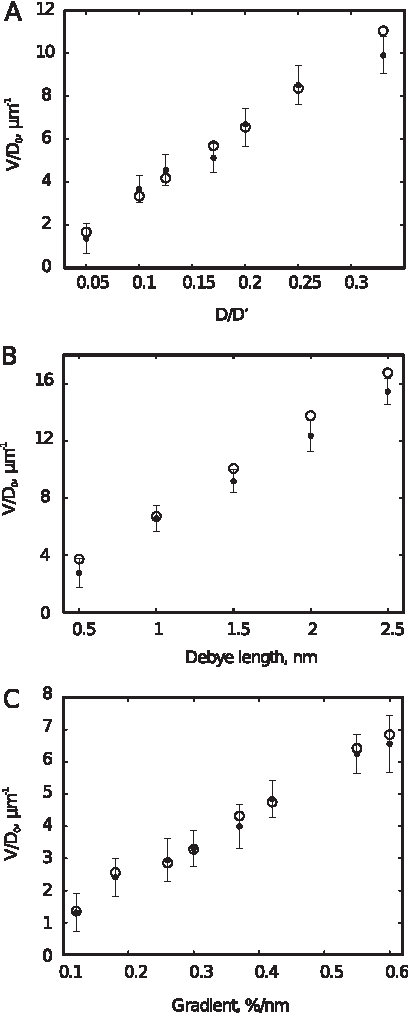
\includegraphics[scale=1.12]{../figures/gradient_MCA_results.pdf}
\end{center}
 \caption[Peptide drift in the gradient of a monovalent lipid (1)]{Peptide drift in the gradient of a monovalent lipid (from \cite{Kiselev2011}). Dependence of the peptide velocity on the peptide diffusion coefficient (A), Debye length (B) and the magnitude of the lipid gradient (C). Simulation results (solid circles) are compared with the values predicted by eq. \eqref{Davide_velocity2} (open circles). In (A), $D_0$ is as defined in subsection \ref{testing_calibration_MCA}. When not otherwise shown in the figure, the peptide diffusion coefficient is 0.2$D_0$ and the lipid gradient is 0.6\%/nm.}
\label{fig:gradient_MCA_results}
\end{figure}

However, to achieve the best fit between the simulation data and eq. \eqref{Davide_velocity2} an empirical prefactor 0.353 (the velocity obtained in the simulations is smaller), identified with the least mean-square method, is required. Presumably, this \mbox{velocity} reduction is due to the effective friction associated with the lipid shell (forming only in the MCA). The details of the effective friction effect are described in the Appendix \ref{effective_friction}.

To further validate the MCA, I also varied the charge of the peptide residues in the non-physiological range between +0.5 and +2.5. The resulting structure does not represent electrostatic properties of the Lys-5 peptide. However, as shown in Fig. \ref{fig:peptide_residue_charge_varying}, the peptide velocities observed in the MCA are in agreement with the prediction of eq. \eqref{Davide_velocity2}. In these simulations the effective charge $Z$ is computed for each value of the residue charge from the MCA and then substituted into eq. \eqref{Davide_velocity2}.

\begin{figure}[!ht]
%\centering
%\scalebox{1.0}[1.0]
\begin{center}
  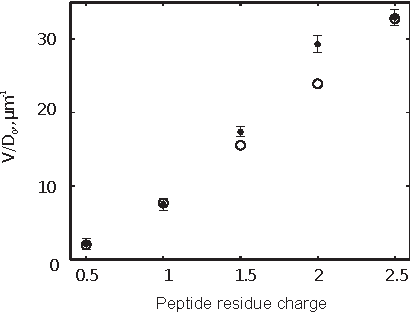
\includegraphics[scale=1.12]{../figures/peptide_residue_charge_varying.pdf}
\end{center}
 \caption[Peptide drift in the gradient of a monovalent lipid (2)]{Peptide drift in the gradient of a monovalent lipid (from \cite{Kiselev2011}). Dependence of the peptide velocity on the peptide residue charge. The peptide diffusion coefficient and the lipid gradient are 0.2$D_0$ and 0.6\%/nm, respectively. Simulation results (filled circles) are compared to the values predicted by eq. \eqref{Davide_velocity2} (open circles).}
\label{fig:peptide_residue_charge_varying}
\end{figure}

Together with the results presented in Fig. \ref{fig:gradient_MCA_results}, this demonstrates that the peptide drift observed in the MCA is fully consistent with the independently derived analytical eqs. \eqref{Davide_velocity2} and \eqref{effective_charge}. 

Moreover, an additional validation of the MCA by comparison with another simulation technique has been performed (see Appendix \ref{additional_validation}).

\begin{figure}[!ht]
%\centering
%\scalebox{1.0}[1.0]
\begin{center}
  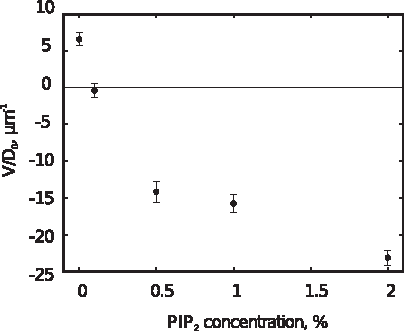
\includegraphics[scale=1.12]{../figures/gradient_MCA_results_pip.pdf}
\end{center}
 \caption[Peptide drift in the gradient of a monovalent lipid with a constant PIP$_2$ concentration]{Peptide drift in the gradient of a monovalent lipid with a constant PIP$_2$ concentration (from \cite{Kiselev2011}). Dependence of the peptide velocity on the PIP$_2$ concentration. The peptide diffusion coefficient is 0.2$D_0$ and the PS lipid gradient is 0.6\%/nm.}
\label{fig:gradient_MCA_results_pip}
\end{figure}

As mentioned above the MCA reproduces only about 30\% of the velocity predicted by eq. \eqref{Davide_velocity2}, however, at the relevant biological conditions the value of the velocity obtained in the MCA is significant. For instance, at $D_p=0.17D_0$ (if $D_0=1$ $\mu$m$^2$/s), Debye length $\lambda$ = 1 nm and the gradient value 0.3 \%/nm the expected velocity value is about 3 $\mu$m/s.

Addition of a small concentration of PIP$_2$ lipids to the membrane with a gradient of PS lipids has an interesting effect on the peptide dynamics. Fig. \ref{fig:gradient_MCA_results_pip} shows that in the absence of PIP$_2$, as expected, the peptide drifts preferably to the area of a high PS density. However, upon addition of the negligible concentration of PIP$_2$ ($\sim$0.1\%), the peptide becomes effectively electro-neutral and shows no systematic drift in either direction. Upon further addition of PIP$_2$ the peptide starts drifting in the opposite direction. Thus, PIP$_2$ lipids significantly change the peptide response to the PS gradient. This effect can be explained by the changes in the total peptide charge at different PIP$_2$ concentrations. As shown in Fig. \ref{fig:ps_pip_competition} and Fig. \ref{fig:total_peptide_charge}, in the physiologically relevant PIP$_2$ range (0--1\%), the number of molecules of PIP$_2$ that are bound to the peptide and, consequently, the total peptide charge change very steeply with the average PIP$_2$ concentration. Therefore, even a small change in the total membrane PIP$_2$ content, e.g. due to signal-induced production or degradation, could drastically change the microenvironment and the dynamics of proteins with polybasic domains.

